\section{Цель работы}
	Научиться описывать поведение компонента распределенной системы с помощью детерминированных конечных автоматов.
		
\section{Порядок выполенения работы}
	\subsection{Устойчевые состояния компонета}
	Из сценария следуют следующие состояния:
	\begin{itemize}
		\item Start - начальное состояние
		\item Pause – состояние паузы
		\item Green – зелёный свет
		\item SwitchToYellow – свет переключается на жёлтый
		\item Yellow – жёлтый свет
		\item SwitchToRed – свет переключается на красный
		\item Red – красный свет
		\item SwitchToGreen – свет переключается на зелёный
		\item End - конечное состояние
	\end{itemize}
		
	\subsection{Машина конечных состояний}
	
		\begin{figure}[h]
			\centering
			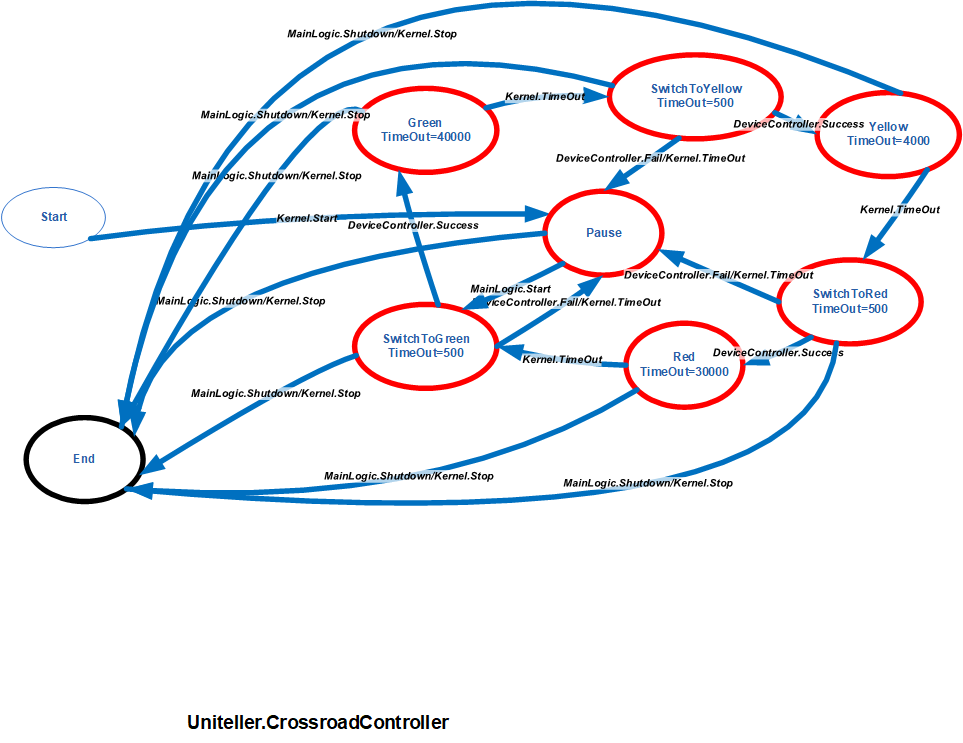
\includegraphics[width=\linewidth]{images/statemachine}
			\caption{Машина состояний}
			\label{fig:statemachine}
		\end{figure}
	
		\FloatBarrier
	\subsection{Декларативное описание машины конечных состояний}
		\lstinputlisting[caption={Описание автомата}]{listings/Uniteller.CrossroadController.utx}
	

\section{Вывод}
	Описано поведение компонента распределенной системы с помощью детерминированных конечных автоматов.